\documentclass[tikz,border=5]{standalone}
\usepackage{tikz}
\usetikzlibrary{shapes.geometric, arrows, positioning, fit, calc}
\usetikzlibrary{arrows,calc,fit}
\tikzset{box/.style={draw, rectangle, rounded corners, thick, node distance=7em, text width=6em, text centered, minimum height=3.5em}}
\tikzset{container/.style={draw, rectangle, dashed, inner sep=2em}}
\tikzset{line/.style={draw, thick, -latex'}}

\begin{document}
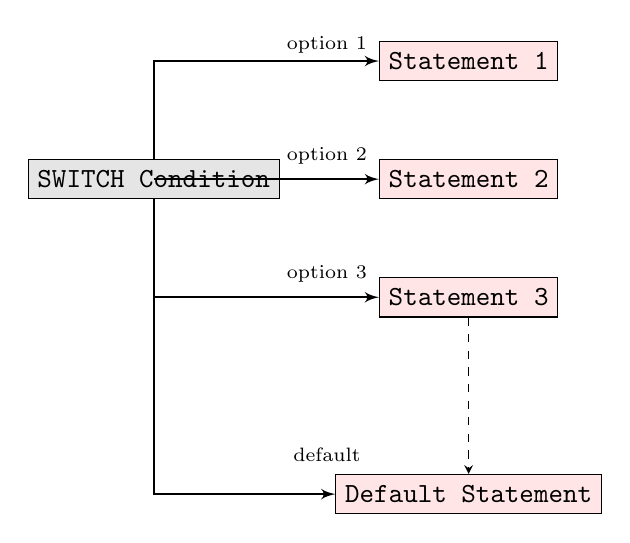
\begin{tikzpicture}
	
	\tikzstyle{statement} = [rectangle, minimum width=0.5cm, minimum height=0.5cm, text centered, draw=black, fill=red!10]
	\tikzstyle{decision} = [rectangle, minimum width=0.5cm, minimum height=0.5cm, text centered, draw=black, fill=black!10]
	\tikzstyle{arrow} = [thick,->,>=stealth]
	\tikzstyle{arrow2} = [dashed,->,>=stealth]
	
	
	\node (statement1) [statement] at (12,6.5) {\texttt{Statement 1}};
	\node (statement2) [statement] at (12,5) {\texttt{Statement 2}};
	\node (statement3) [statement] at (12,3.5) {\texttt{Statement 3}};
	\node (default) [statement] at (12, 1) 
	{\texttt{Default Statement}};
	\node (decision) [decision] at (8, 5) 
	{\texttt{SWITCH Condition}};
	
    \path [line] (decision) |- (default);
    \path [line] (decision) |- (statement1);
    \path [line] (decision) |- (statement2);
    \path [line] (decision) |- (statement3);
    \draw [arrow2] (statement3) -- (default);
    
    \node at (10.2, 6.7) {\scriptsize option 1};
    \node at (10.2, 5.3) {\scriptsize option 2};
    \node at (10.2, 3.8) {\scriptsize option 3};
    \node at (10.2, 1.5) {\scriptsize default};
    
    

	
	
\end{tikzpicture}
\end{document}
